\section{Молекулярно-статистический метод расчета процесса ректификации}



\subsection{Молекулярно-статистические методы и программные пакеты}

В настоящее время молекулярно~-- статистические методы находят широкое применение в научных исследованиях в различных отраслях. Данные методы позволяют на молекулярном уровне исследовать свойства веществ, а также процессов происходящих на молекулярном уровне. Для проведения моделирования разработано множество пакетов программ, отличающихся функциональностью и условиями предоставления программ \cite{wiki_progs}. Множество программных продуктов создано под коммерческой лицензией, например Material Studio \cite{material_studio} , Materials Science Suite \cite{shedinger} и т.~д. Данные программные продукты нацелены на широкое применение во многих областях, что зачастую плохо сказывается на производительности их вычислений. Однако в них есть свой интерфейс пользователя, что существенно снижает порог вхождения и простоту для конченного потребителя.

Если сравнивать два подхода молекулярного моделирования: метод молекулярной динамики и метод Монте~-- Карло, и их модификации, то наибольшее распространение получил метод молекулярной динамики. В первую очередь это связано с тем, что данный метод позволяет получить кинетические характеристики, такие как коэффициенты диффузии, вязкости и т.~д. Также сравнивая алгоритмы расчета, метод молекулярной динамики позволяет более эффективно использовать параллельные расчеты на нескольких вычислительных ядрах. Данный факт также способствовал большему распространению вычислений с использованием метода молекулярной динамики. Среди программ с открытым исходным кодом можно выделить gromacs \cite{Berendsen1995,Pronk2013,Abraham2015} и LAMMPS \cite{Plimpton1995,Thompson2009} . Данные программы получили широкое распространение за счет открытого исходного кода и большого количества заинтересованных разработчиков, что привело к отличной вычислительной производительности, в том числе на специфическом оборудовании. 

Метод Монте-Карло при моделировании классических (не квантовых систем) также обладает своими преимуществами. Так намного проще реализовано вычисление химического потенциала системы, что позволяет проще производить вычисления фазового равновесия. Так, для вычисления фазового равновесия разработан ансамбль Гиббса \cite{Panagiotopoulos1987,Orkoulas1994}. Среди программного обеспечения с открытым исходным кодом можно выделить towhee \cite{Martin2013}. Данная программа изначально разрабатывалась для моделирования паро~-- жидкостного равновесия и содержит множество наборов параметров для моделирования. Недостатком данного пакета является то, что во времена начала разработки данной программы не были распространены многопроцессорные компьютеры и многоядерные процессоры. Таким образом данный пакет не позволяет в полной мере использовать все достоинства многопоточного вычисления.



\subsection{Многопоточное вычисление и программно-аппаратная технология CUDA}
Использование молекулярно-статистических методов непосредственно связано с развитием вычислительных технологий еще с разработки первых ЭВМ \cite{Allen1988}. Рассматривая развитие персональных компьютеров можно сказать, что увеличение вычислительных мощностей до середины 2000-х годов продолжалось в большей степени за счет наращивания частоты процессора. Однако накладываемые технологические ограничения не позволили превысить номинальную частоту в 4 ГГц для центрального процессора. В 2005 году на рынок выпускают процессор, содержащий два ядра. В дальнейшем происходит тенденция к наращиванию количества ядер в процессоре. Параллельно с этим развиваются программные средства, позволяющие использовать множество потоков для вычисления.

В 2008 году была представлена программно аппаратная технология CUDA использующая для вычислений процессор видеокарты. Отличие от центрального процессора заключается в том, что видеокарта имеет множество специализированных процессоров, их количество в современных видеокартах достигает нескольких тысяч. Данная технология позволяет увеличить производительность для отдельных задач в несколько десятков и сотен раз. Позже появилась аналогичная технология OpenCL, не привязанная к оборудованию конкретного производителя.

В задачах молекулярной динамики использование видеокарт для расчета приводит к увеличению производительности в 10 раз по сравнению с использованием только центрального процессора. Данные технологии реализованы во многих программных продуктах \cite{wiki_progs}.

\subsection{Ансамбль Гиббса} \label{p.gibbs}
Для того чтобы две фазы (обозначенные I и II) находились в равновесии необходимо выполнение следующих условий:
\begin{itemize}
	\item термическое равновесие (равенство температур) $T^I = T^{II}$;
	\item механическое равновесие (равенство давлений) $p^I = p^{II}$;
	\item химическое равновесие (равенство химического потенциала каждого из компонентов) $\mu_i^I = \mu_i^{II}$.
\end{itemize}

Метод ансамбля Гиббса предусматривает моделирование двух ячеек с молекулами, предусматривающие три типа случайных изменений конфигурации:
\begin{itemize}
	\item перемещение молекулы внутри каждой ячейки (перемещение, вращение, изменение внутренней геометрии молекулы);
	\item изменение объемов каждой из ячейки;
	\item перемещение молекул между ячейками.
\end{itemize}
После каждого изменения конфигурации рассчитывается вероятность принятия или отклонения данного изменения. После значительного количества перемещений между двумя ячейками устанавливается равновесие.


\subsection{Алгоритм расчета ректификации}
Согласно предлагаемому методу, ректификационная колонна делится на участки, аналогичные теоретическим тарелкам (теоретическим ступеням). Каждая из тарелок делится на две ячейки, которые соответствуют газовой и жидкой фазам. Суммарный объем газовой и жидкой фазы на каждой из тарелок остается постоянным. С точки зрения конструкции колонны данный указанный суммарный объем характеризует объем колонны между тарелками.При проектировании могут применяться колонны с переменным диаметром, что обеспечивает равномерность газовой фазы по высоте колонны. Таким образом в алгоритме суммарный объем каждой из ячеек может быть задан любой, однако он не меняется во время моделирования.

На тарелке между газовой и жидкой фазами устанавливается фазовое равновесие, рассчитываемое методом ансамбля Гиббса (раздел \ref{p.gibbs}). После достижения фазового равновесия жидкость уходит на нижнюю тарелку, пар поднимается на верхнюю. Молекулы переносят свою энергию (кинетическую и потенциальную) и, исходя из этой энергии, проводится пересчет температуры на новой тарелке. И расчетный цикл повторяется и заново рассчитывается фазовое равновесие. 

Таким образом в колонне можно проследить за материальными (количество молекул каждого из веществ) и тепловыми потоками (энергия молекул). Также в колонне можно выделить внешние материальные и тепловые потоки: приток молекул с исходной смесью, и флегмой, уход молекул с дистиллятом и кубовым остатком.

Блок-схема алгоритма расчета представлена на рисунке \ref{fig:alg_scheme}. На первом этапе проводится чтение исходных данных для моделирования. Далее рассчитываются свойства входящих материальных потоков. При условии, что колонна работает в стационарном режиме, свойства входящих потоков не должны изменяться. И данную процедуру необходимо провести только один раз на начальном этапе. Однако можно предусмотреть динамическое изменение исходного состава. В этом случае вычисление входящих материальных потоков необходимо включить в расчетный цикл.

\begin{figure}
	\begin{center}
		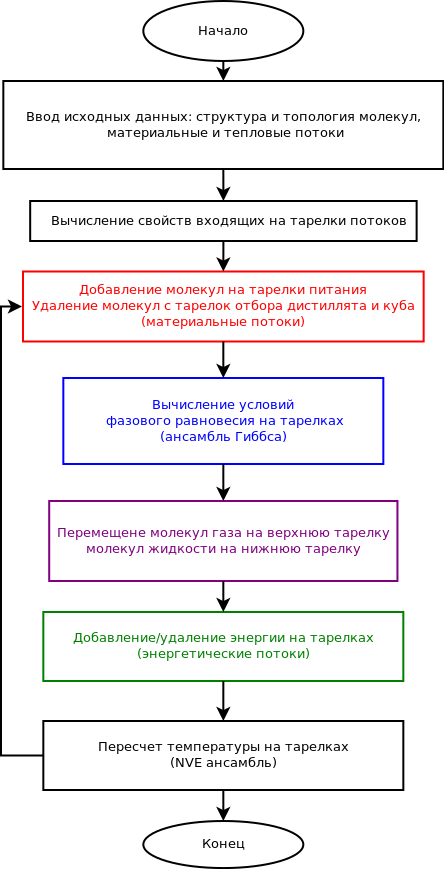
\includegraphics[width=0.5\textwidth]{scheme.png}
	\end{center}
	\caption{Блок-схема алгоритма расчета} \label{fig:alg_scheme}
\end{figure}

Далее рассчитываются внешние материальные потоки (красный блок): добавляется заданное количество молекул на тарелку питания, рассчитывается количество молекул во флегме, а также количество молекул выводимых из куба.

Далее вычисляются условия фазового равновесия на каждой тарелке с использованием ансамбля Гиббса (синий блок).

После установления фазового равновесия на всех тарелках происходит обмен молекулам между тарелками. Жидкая фаза переходит на нижнюю тарелку, газовая фаза переходит на верхнюю тарелку (фиолетовый блок).

На каждую из тарелок можно вводить дополнительные энергетические потоки: подогрев куба колонны, введение дополнительных змеевиков охлаждения и т.д. (зеленый блок)

После перемещения молекул на каждой из тарелок вычисляется температура по внутренней энергии газовой и жидкой фаз (черный блок). Суммарная энергия молекул на тарелке высчитывается как кинетическая и потенциальная энергия молекул газовой и жидкой фаз. Кинетическая энергия может быть вычислена из температуры на тарелке, потенциальная --- как сумма межмолекулярного и внутримолекулярного (потенциал валентных и торсионных углов и т.д.) взаимодействия.
Новая температура на тарелке может быть вычислена из энергии молекул на тарелке с использованием ансамбля с постоянным количеством молекул, объемом и энергией $NVE$ \cite{Lustig1998}.

Альтернативный алгоритм определения температуры основан на на одновременном изменении температуры во время вычисления фазового равновесия. В данном случае блок добавления энергии будет выполнен раньше, чем расчет условий фазового равновесия. Во время вычисления фазового равновесия температура на тарелке будет динамически изменяться таким образом, чтобы на энергия системы была равна сумме энергий поступающих на тарелку молекул с газовой и жидкой фазой, и энергетических потоков. Выбор конкретной из описанных выше  реализаций алгоритма определения температуры будет осуществляться на этапе программирования.
 
Далее алгоритм циклически повторяется до достижения условия стационарности, или любого другого заданного условия. Например при периодической ректификации могут быть задано количество оставшейся жидкости в кубе, при этом будет исследован неравновесный процесс.
 
На рисунке \ref{fig:plate_scheme} представлена схематическое распределение потоков в ректификационной колонне. Цвет стрелок и текста соответствует различным этапам алгоритма, представленного на рисунке \ref{fig:alg_scheme}


\begin{figure}[h]
	\begin{center}
		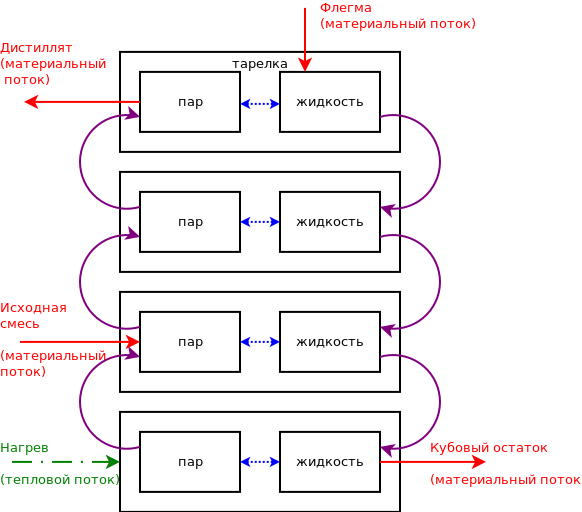
\includegraphics[width=0.7\textwidth]{column.png}
	\end{center}
	\caption{Схематическое изображение ректификационной колонны (цвет соответствует различным этапам, представленным на рисунке \ref{fig:alg_scheme})} \label{fig:plate_scheme}
\end{figure}

Усреднение свойств смеси на тарелках и выходных потоках (концентрации, температуры, давления и т.д.) проводится после установления стационарности. Достижение стационарности можно отследить по неизменности составов и количества молекул на каждой тарелке.

Достоинства предлагаемого алгоритма расчета:
\begin{itemize}
	\item не нужно заранее знать фазовое равновесие разделяемых компонентов;
	\item расчет ведется с учетом непостоянства мольных потоков по колонне;
	\item возможность исследования как непрерывной так и периодической ректификации;
\end{itemize}
Недостатками является то, что данный метод не учитывает эффективность тарельчатых устройств реальных аппаратов, обусловленной гидродинамической обстановкой. Данную проблему можно решить в будущем.


